% !TeX encoding = UTF-8

\chapter{实验设计与结果分析}

\section{实验环境与基准方法}

本节在公开图像分类基准数据集上对所提自适应聚合方法进行对比验证，主要对比方法包括经典联邦平均算法 FedAvg\cite{mcmahan2017fedavg} 及固定噪声尺度差分隐私基线 DP-FedAvg。

\section{收敛性能曲线分析}

按照规范 2.4.1 节要求，插图一般随文编排、先见文字后见图；图序与图题居中排于图的下方，曲线图纵横坐标应标注“量、标准规定符号、单位”，且不同曲线采用不同形状标识符区分。如图~\ref{fig:conv-curve} 所示，本文方法在前期通信轮次中即展现出更快的收敛速率与更平滑的泛化曲线。

\begin{figure}[htbp]
  \centering
  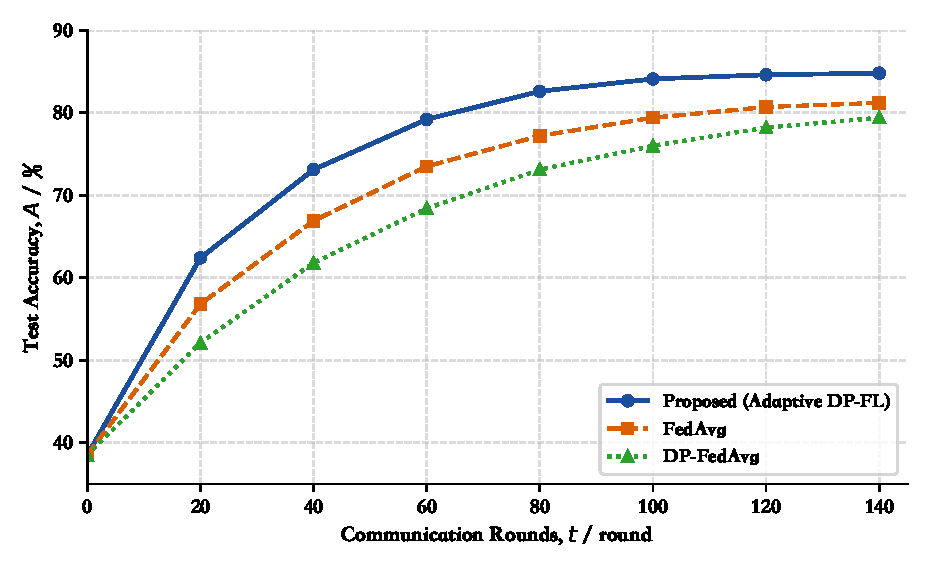
\includegraphics[width=0.78\textwidth]{figures/demo-curve.pdf}
  \caption{不同聚合算法在异构数据下的测试准确率收敛曲线}
  \label{fig:conv-curve}
\end{figure}

图~\ref{fig:subfigs} 展示了双子图并排排版示例，图序与子图编号均自动匹配五号宋体规范要求。

\begin{figure}[htbp]
  \centering
  \begin{subfigure}[b]{0.47\textwidth}
    \centering
    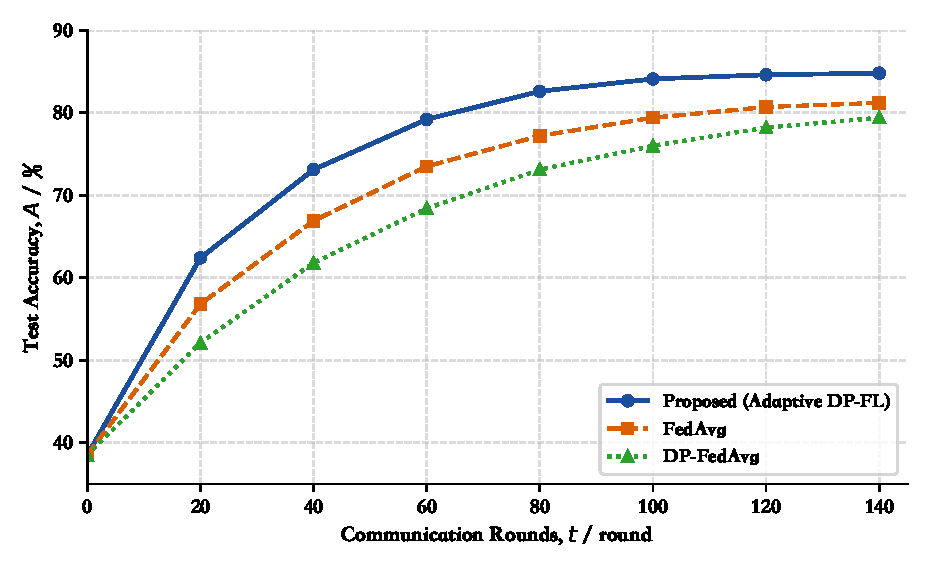
\includegraphics[width=\textwidth]{figures/demo-curve.pdf}
    \caption{隐私预算 $\varepsilon = 4.0$}
    \label{fig:sub-a}
  \end{subfigure}
  \hfill
  \begin{subfigure}[b]{0.47\textwidth}
    \centering
    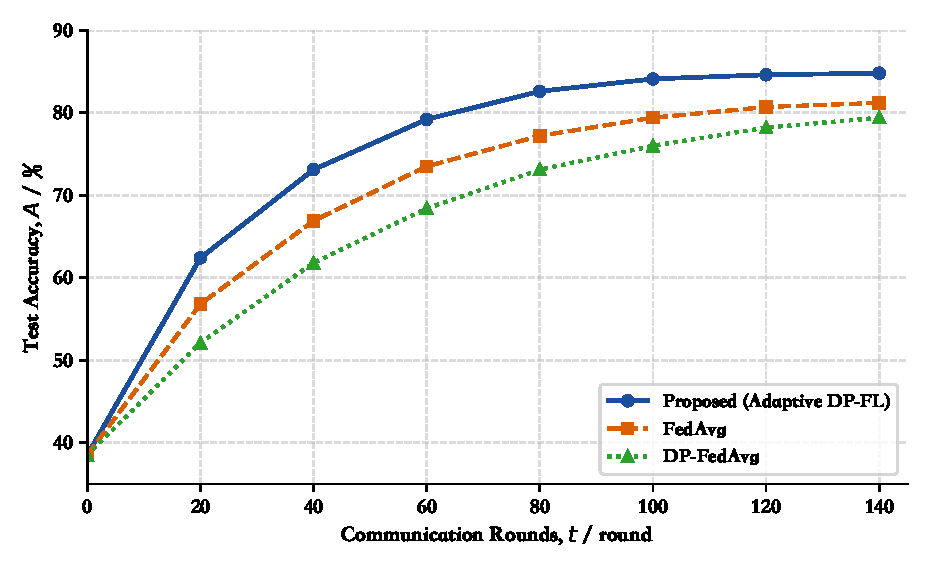
\includegraphics[width=\textwidth]{figures/demo-curve.pdf}
    \caption{隐私预算 $\varepsilon = 8.0$}
    \label{fig:sub-b}
  \end{subfigure}
  \caption{不同隐私预算约束下的算法性能对比}
  \label{fig:subfigs}
\end{figure}

\section{消融实验与讨论}

表~\ref{tab:ablation} 汇总了各核心模块对最终测试准确率与通信轮次的贡献。移除动态隐私预算分配或梯度一致性加权均会导致模型准确率明显下降，表明两个模块在非独立同分布与隐私噪声耦合场景下具有良好互补性\cite{chendengyuan2000}。

\begin{table}[htbp]
  \centering
  \caption{核心模块消融实验结果对比}
  \label{tab:ablation}
  \begin{tabular}{@{}l c c c@{}}
    \toprule
    方法变体 & 最终准确率 / \% & 达标通信轮次 / 轮 & 相对增益 / \% \\
    \midrule
    DP-FedAvg（基线） & 79.4 & 145 & — \\
    + 梯度一致性自适应加权 & 82.6 & 112 & +3.2 \\
    + 分阶段动态隐私预算 & 81.9 & 118 & +2.5 \\
    完整方法（本文） & \textbf{84.8} & \textbf{98} & \textbf{+5.4} \\
    \bottomrule
  \end{tabular}
\end{table}
